\documentclass[11pt]{article}
\usepackage[margin=1in]{geometry}
\usepackage{graphicx}
\usepackage{booktabs}
\usepackage{subcaption}
\usepackage{xcolor}
\usepackage{enumitem}
\usepackage{titlesec}
\usepackage[hidelinks]{hyperref}
\usepackage{parskip}

\definecolor{accent}{RGB}{20,80,140}
\definecolor{soft}{RGB}{90,90,90}
\titleformat{\section}{\Large\bfseries\color{accent}}{\thesection}{0.6em}{}
\titleformat{\subsection}{\large\bfseries\color{accent}}{\thesubsection}{0.6em}{}
\newcommand{\code}[1]{\texttt{\small #1}}
\graphicspath{{figures/}}

\title{\vspace{-1.5cm}\textbf{Explainable-AI Evaluation for Construction-Safety\\Vision-Language Models}\\[0.3cm]
\large A Two-Week Feasibility Pilot and the Case for Scale-Up}
\author{Research advised by Professor Mustafa Abdallah}
\date{Pilot complete --- \today}

\begin{document}
\maketitle
\vspace{-0.8cm}

\begin{abstract}
\noindent This report documents a completed feasibility pilot testing whether Professor Abdallah's
six-metric explainable-AI (XAI) evaluation framework --- Descriptive Accuracy, Sparsity, Stability,
Efficiency, Robustness, and Completeness, originally built and validated on tabular
network-intrusion-detection models --- transfers to a Vision-Language Model (VLM) making visual
safety judgments on construction sites. Using Florence-2-base-ft (231M parameters, a single RTX 3070)
on 163 images from the ConstructionSite dataset, all six metrics ran end-to-end and produced genuine,
interpretable signal. \textbf{The framework transfers, but required two real adaptations, not zero
changes.} The pilot also surfaced a small number of cross-cutting mechanisms --- most importantly, that
on Florence-2 the safety judgment is ultimately computed by hand-written geometric code rather than by
the model, which means some metrics partly measure the proxy rather than the model. This report
presents the method, results, findings, and honest limitations, and motivates a phased scale-up whose
central goal is to make the metrics measure \emph{model faithfulness}.
\end{abstract}

\section{Executive Summary}

\textbf{The question.} Does a six-metric XAI evaluation framework built for tabular models transfer to
a VLM making visual judgments? \textbf{The answer: yes, with two quantified adaptations.}

\begin{enumerate}[leftmargin=*,itemsep=2pt]
\item \textbf{Florence-2 has no native question-answering token.} Each safety rule was reframed as an
open-vocabulary grounding query (detect ``worker'' and the relevant safety object, then apply a
per-worker coverage check) rather than a literal yes/no question.
\item \textbf{The first version of that proxy barely worked} --- 3.0\% sensitivity, effectively a
constant ``compliant'' classifier. A person-relative redesign, mirroring the dataset's own per-worker
labels, produced a \textbf{9$\times$ sensitivity gain to 27.0\%}.
\end{enumerate}

With both adaptations in place, the six metrics produced the headline numbers in
Table~\ref{tab:headline}. The findings that matter more than any single number are cross-cutting: one
region-ranking choice weakens three metrics at once on the PPE rules; a stable answer can hide a
fully-drifted explanation; and, most consequentially for the next phase, the model does not actually
make the safety judgment --- our geometric code does.

\begin{table}[h]
\centering
\begin{tabular}{lr}
\toprule
\textbf{Metric} & \textbf{Result (163 samples)} \\
\midrule
Descriptive accuracy (masking the top region flips the answer) & 36.2\% \\
Visual sparsity (top-5-of-576-cell attention mass) & 0.108 \\
Stability (3-run sampled answer agreement) & 77.5\% \\
Robustness, Level 1 (survives blur / low-light / occlusion / contrast) & 80.7\% \\
Bounded completeness (top region masking is load-bearing) & 43.6\% \\
Efficiency (full six-metric pipeline @ $n{=}1{,}000$) & $\sim$0.5 GPU-hours \\
\bottomrule
\end{tabular}
\caption{Headline results. All six metrics ran end-to-end and produced interpretable signal.}
\label{tab:headline}
\end{table}

\section{Motivation and Research Question}

Professor Abdallah's XAI framework evaluates black-box explanations along six axes and was validated on
tabular network-intrusion-detection DNNs, where a ``feature'' is a scalar column. Construction-safety
monitoring with VLMs is a very different setting: the input is an image plus a text prompt, and an
``explanation'' is a spatial region rather than a feature weight. The research question is whether the
framework's \emph{structure} survives that move --- and, where it does not transfer for free, what
minimal adaptation makes each metric meaningful again. A feasibility pilot is the right instrument for
this: it surfaces the adaptations a full study would otherwise discover the hard way.

\section{Dataset and Task}

The pilot uses the ConstructionSite dataset (10,013 images; a 3,004-image test split was used). Each
image carries annotator-written violation fields for four safety rules:

\begin{table}[h]
\centering
\begin{tabular}{llp{6.4cm}}
\toprule
\textbf{Rule} & \textbf{Hazard class} & \textbf{What it checks} \\
\midrule
rule\_1 & ppe\_violation & Basic PPE present (hard hat / hi-vis vest) \\
rule\_2 & fall\_hazard & Fall protection (harness / lanyard) at height \\
rule\_3 & fall\_hazard & Edge protection (guardrail) at height / excavation edges \\
rule\_4 & struck\_by\_risk & Worker inside an excavator's blind spot / swing radius \\
\midrule
(none) & compliant & Every applicable safety requirement satisfied \\
\bottomrule
\end{tabular}
\caption{The four safety rules and the hazard classes they map to.}
\label{tab:rules}
\end{table}

A balanced 163-image subset was drawn (50 each for three classes; \code{struck\_by\_risk} capped at 13
--- a labeling artifact discussed in Section~\ref{sec:limits}). Ground truth comes from the dataset's
own annotations; the model is then tested on whether it reaches the same judgment, and whether the
region it used is a trustworthy explanation.

\section{Model and the Grounding-Proxy Adaptation}

Florence-2-base-ft was chosen as a lightweight, region-native baseline: it runs on an 8\,GB consumer
GPU and produces bounding boxes directly, so a candidate ``explanation'' (a box) falls out of the model
without a separate localization step. Its limitation is central: \textbf{it has no free-form
question-answering task token}. A safety question therefore cannot be asked literally.

The adaptation converts each rule into open-vocabulary detection calls and derives the answer
geometrically. For a PPE rule: detect ``worker'' boxes and ``hard hat'' boxes, then mark the scene
\emph{compliant} only if every detected worker has a nearby safety-object box (Figure~\ref{fig:baseline}).
A first version that merely asked ``does a hard hat exist anywhere in the image?'' failed at 3.0\%
sensitivity, because multi-worker scenes almost always contain \emph{some} hard hat. The person-relative
redesign fixed this (27.0\% sensitivity).

\begin{figure}[h]
\centering
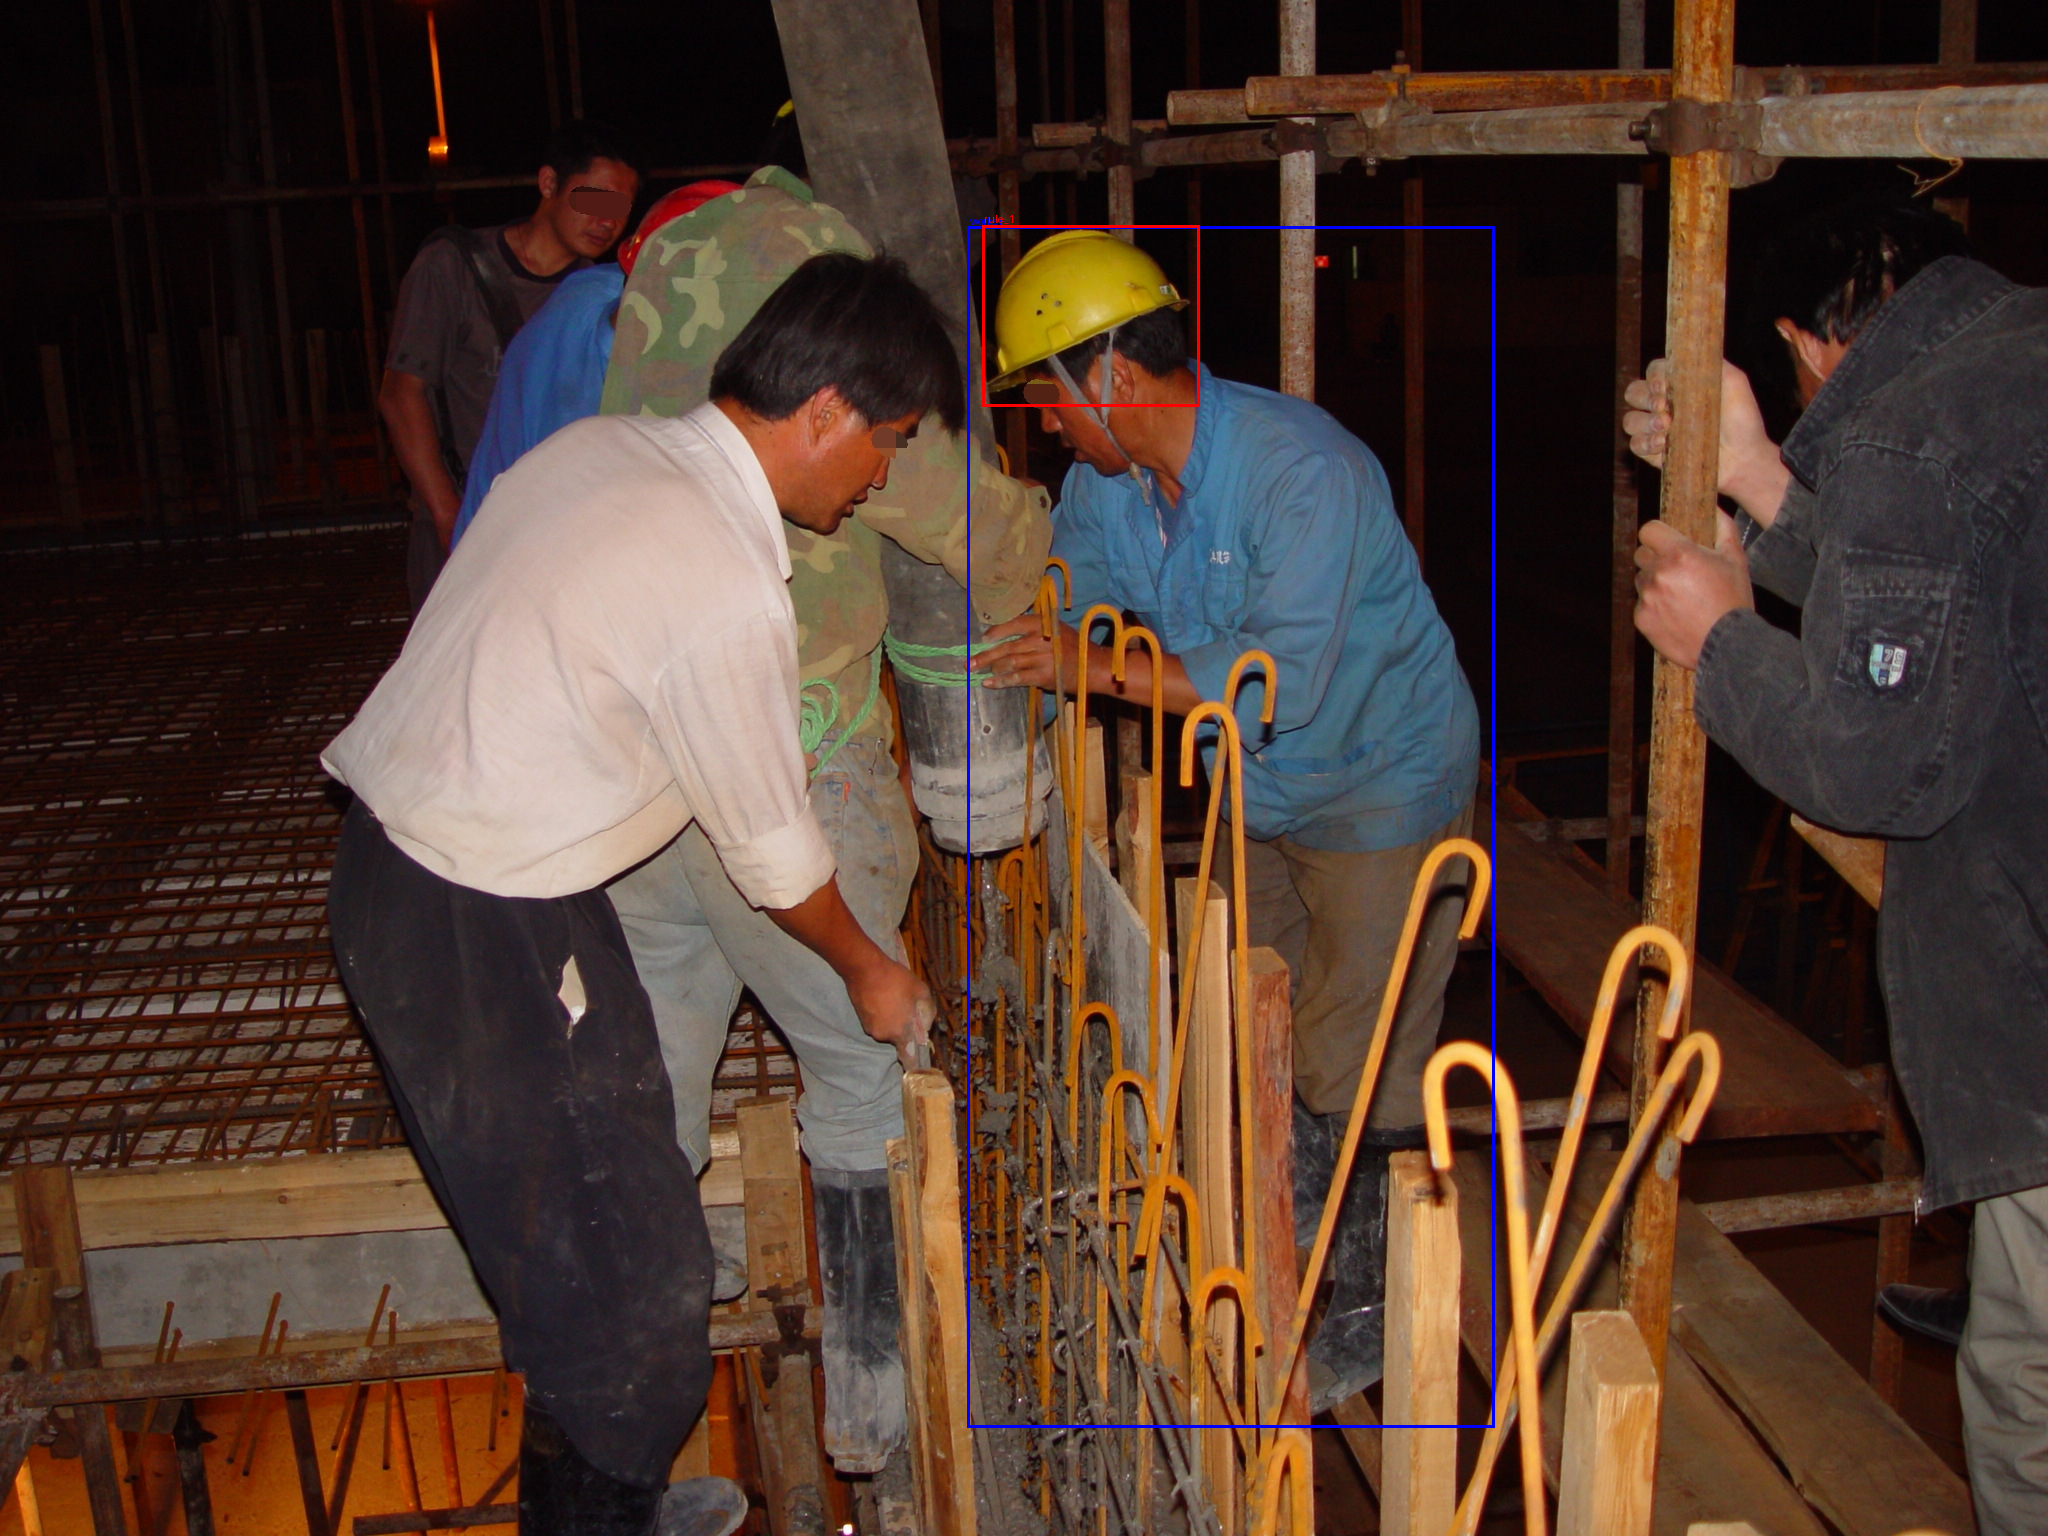
\includegraphics[width=0.55\linewidth]{baseline_grounding.png}
\caption{The grounding-proxy adaptation working: a ``hard hat'' query correctly localized on a worker's
head. This mechanism underlies the 3.0\%$\to$27.0\% sensitivity gain.}
\label{fig:baseline}
\end{figure}

\textbf{A caveat that shapes the entire scale-up:} Florence-2 never makes the safety judgment. It only
locates objects; a hand-written geometric rule (per-worker coverage within a fixed pixel-distance
threshold) produces the compliant/violation answer. Several metrics therefore partly measure the
sensitivity of that geometric proxy rather than the model's own reasoning --- the single most important
reason to add a native question-answering model in the full study (Section~\ref{sec:scaleup}).

\section{System Architecture}

The pipeline is a sequence of stages that each build on the last: environment setup $\to$ balanced
sample selection $\to$ baseline grounding inference $\to$ region standardization (rank candidate boxes
into an ordered list and provide a masking primitive) $\to$ the five per-sample metrics plus the
efficiency accounting $\to$ bounded completeness (a roll-up over two earlier stages) $\to$ a
cross-metric summary. Every metric consumes the region-standardization layer, which is why one choice
made there (how to rank candidate regions) propagates into several metrics at once --- a fact that
becomes the pilot's central cross-cutting finding.

\section{The Six Metrics: Method and Results}

\subsection{Descriptive Accuracy --- does masking the top region change the answer?}
Mask the top-ranked explanation region, re-run, and check whether the answer flips; a genuinely
load-bearing region should flip it. Headline: \textbf{36.2\%} (top-1), 35.0\% (top-1+2).
Figure~\ref{fig:daflip} shows a clean case: masking the excavator box in a proximity rule removes half
the proximity comparison and flips \code{hazard}$\to$\code{safe}. The metric's main weakness is that it
is confounded by the proxy it sits on: rules whose proxy barely discriminates have little for masking to
disrupt.

\begin{figure}[h]
\centering
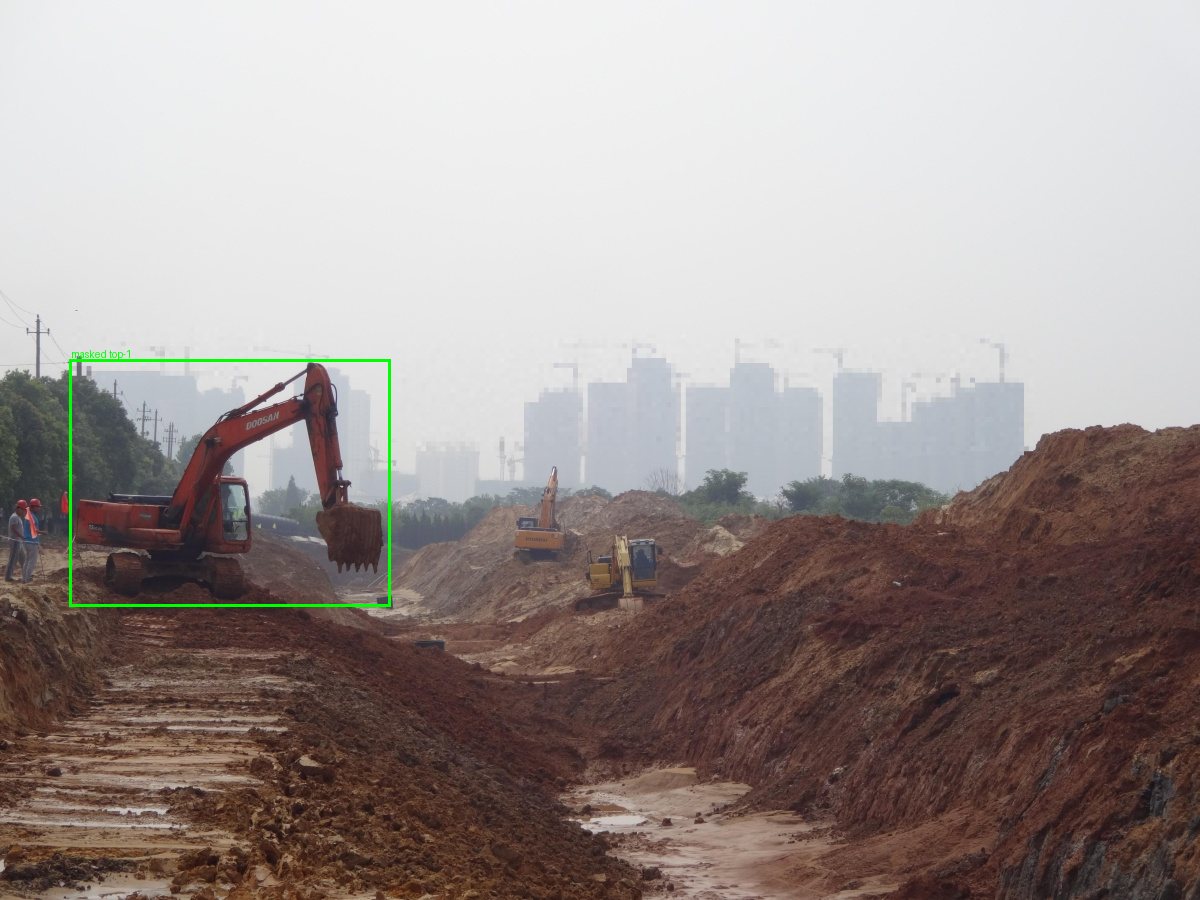
\includegraphics[width=0.5\linewidth]{da_flip.png}
\caption{Descriptive accuracy behaving as designed: masking the top-ranked region (here the excavator in
a struck-by-risk sample) changes the model's judgment for a reason that tracks the safety concept.}
\label{fig:daflip}
\end{figure}

\subsection{Visual Sparsity --- how concentrated is the attention?}
Because the planned attention-rollout method assumes a single-modality encoder and Florence-2 fuses
image and text tokens in one shared self-attention stack, rollout was verified inapplicable and
replaced with decoder$\to$encoder cross-attention. Headline top-5-of-576-cell mass ratio: \textbf{0.108}.
The central finding is a \emph{confound}: concentration correlates $-0.70$ with object size --- a small
hard hat looks ``focused'' simply because it covers few cells (Figure~\ref{fig:sparsity}). Cross-rule
sparsity comparisons are invalid without a size control.

\begin{figure}[h]
\centering
\begin{subfigure}{0.44\linewidth}\centering
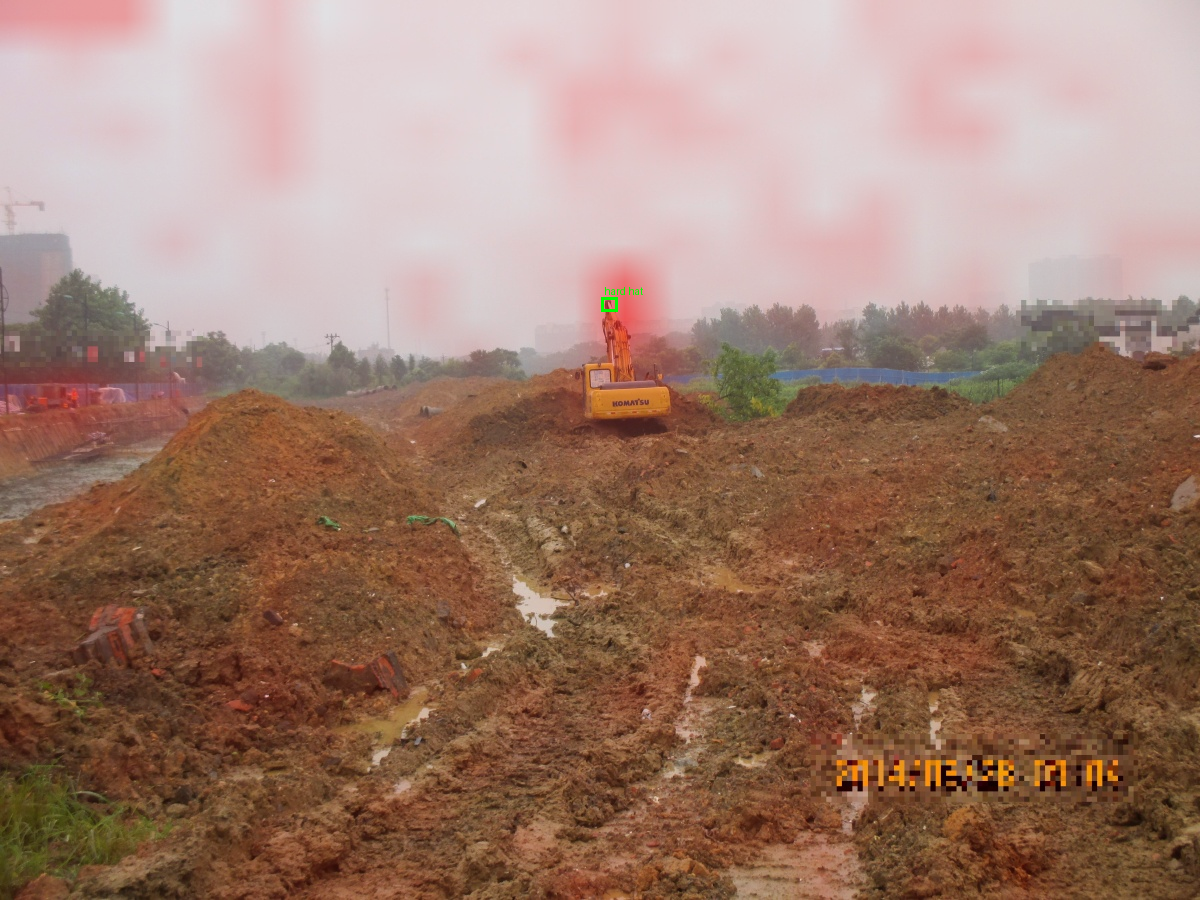
\includegraphics[width=\linewidth]{sparsity_focused.png}
\caption{Small hard hat: a sharp, concentrated hotspot.}
\end{subfigure}\hfill
\begin{subfigure}{0.44\linewidth}\centering
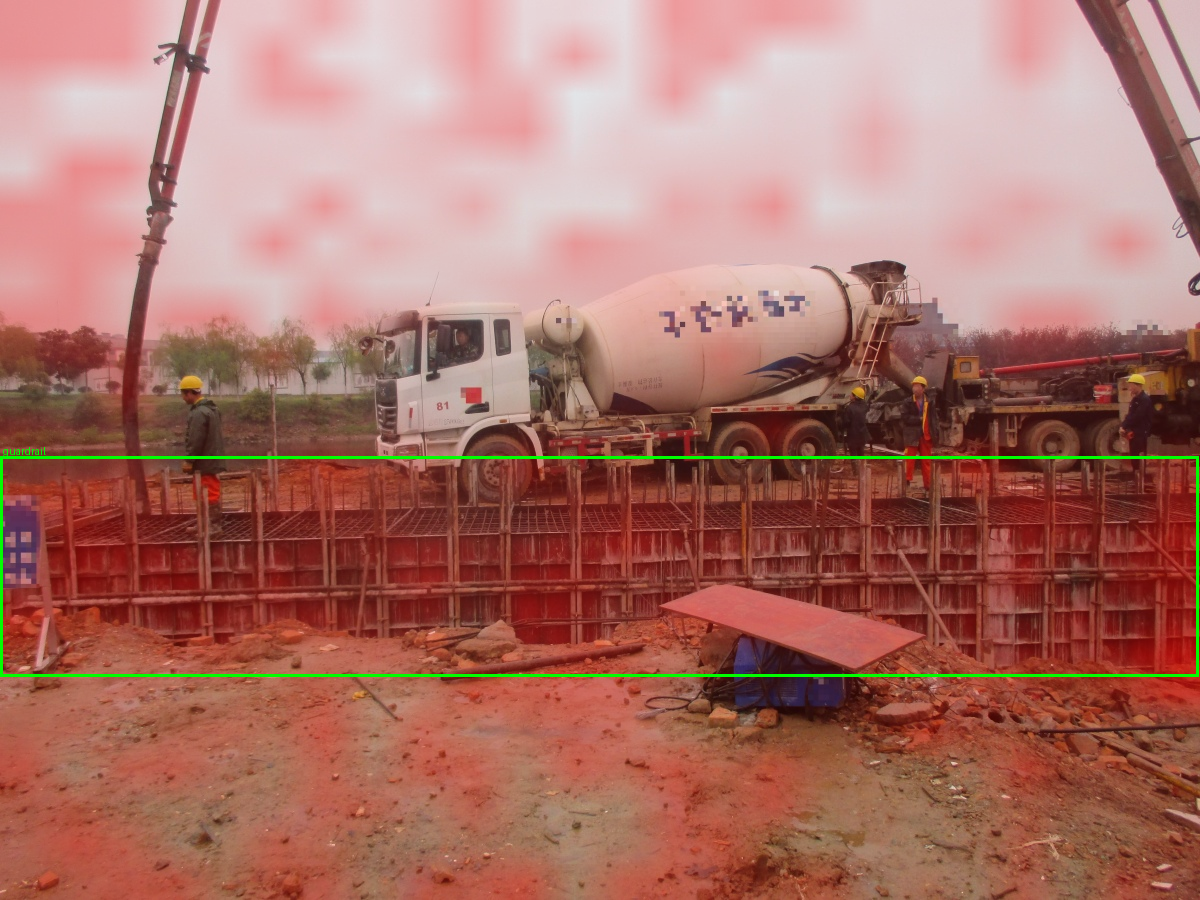
\includegraphics[width=\linewidth]{sparsity_scattered.png}
\caption{Large guardrail: attention spread across the frame.}
\end{subfigure}
\caption{The size confound made visible: concentration tracks object footprint, not explanation quality.}
\label{fig:sparsity}
\end{figure}

\subsection{Stability --- does the explanation stay put across reruns?}
Deterministic reruns would be trivially 100\% stable, so stability is measured under stochastic
decoding, confirmed non-vacuous (answer agreement 0.775, not 1.0). Headline object-box overlap
\textbf{0.602}. The finding: a healthy-looking top-region overlap (0.667) \emph{hid} the instability of
the actual safety object (rule\_1 hard hat only 0.499 vs.\ rule\_4 excavator 0.922). Small, body-worn
PPE items are least stable --- partly a genuine effect and partly the same size bias, since IoU
penalizes small boxes. Figure~\ref{fig:stability} overlays three reruns' top boxes.

\begin{figure}[h]
\centering
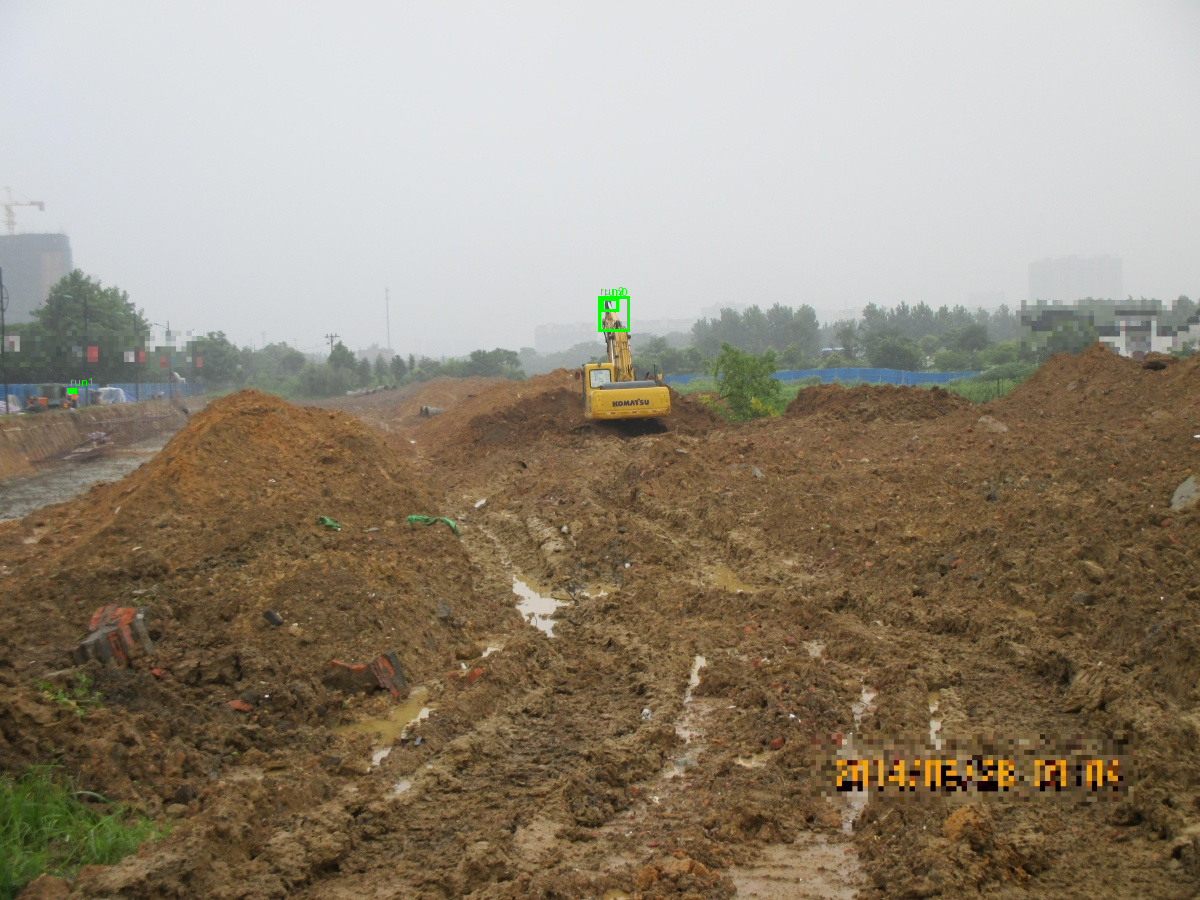
\includegraphics[width=0.5\linewidth]{stability_reruns.png}
\caption{Three stochastic reruns overlaid. The large top-ranked (worker) boxes sit almost exactly on top
of each other; the small hard-hat box the rule is actually about is far less stable underneath.}
\label{fig:stability}
\end{figure}

\subsection{Robustness --- do answer and explanation survive perturbation?}
Four image perturbations plus prompt rewording, under deterministic decoding to isolate perturbation
from sampling noise. Level-1 answer survival: \textbf{80.7\%}. \textbf{This chapter contains the pilot's
strongest single result:} in 28.3\% of cases where the final answer did \emph{not} change, the model's
evidence box nonetheless drifted to something unrelated (Figure~\ref{fig:drift}). An answer-level metric
alone would certify these as perfectly robust. This is direct evidence that answer-level metrics are
necessary but not sufficient --- and it motivates reporting answer-level and explanation-level
robustness as two never-blended numbers.

\begin{figure}[h]
\centering
\begin{subfigure}{0.44\linewidth}\centering
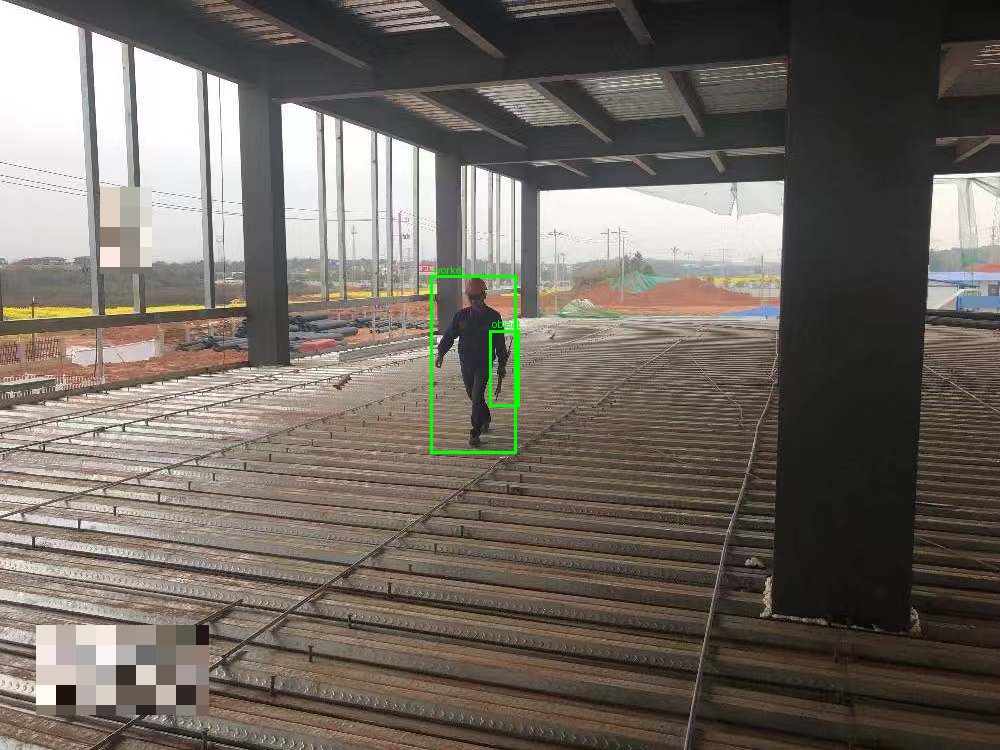
\includegraphics[width=\linewidth]{drift_before.png}
\caption{Before: the worker's evidence box, fully visible.}
\end{subfigure}\hfill
\begin{subfigure}{0.44\linewidth}\centering
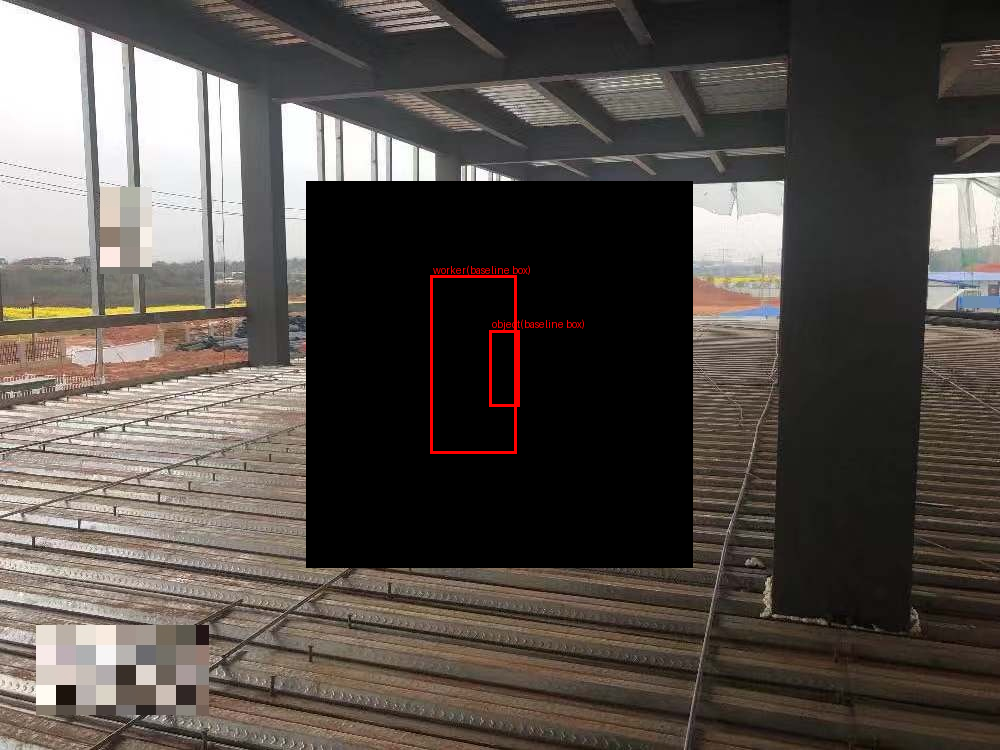
\includegraphics[width=\linewidth]{drift_after.png}
\caption{After occlusion: answer unchanged, but the evidence box relocated almost entirely (IoU 0.005).}
\end{subfigure}
\caption{The centerpiece finding: a stable answer hiding a fully-drifted explanation.}
\label{fig:drift}
\end{figure}

\subsection{Bounded Completeness --- is the top region actually necessary?}
A necessity test: does removing the top region force the model to change its answer? Headline
\textbf{43.6\%} supported. The metric is built from the descriptive-accuracy signal (so the two are not
independent confirmations), and its by-rule pattern is the clearest measurement of the area-ranking
confound (Section~\ref{sec:findings}). The pilot also ran an extra 159-rerun check that revealed a small
inflation from a fallback artifact (Figure~\ref{fig:completeness}), correcting the number from 43.6\% to
41.7\% --- an example of the rigor a full study should standardize.

\begin{figure}[h]
\centering
\begin{subfigure}{0.44\linewidth}\centering
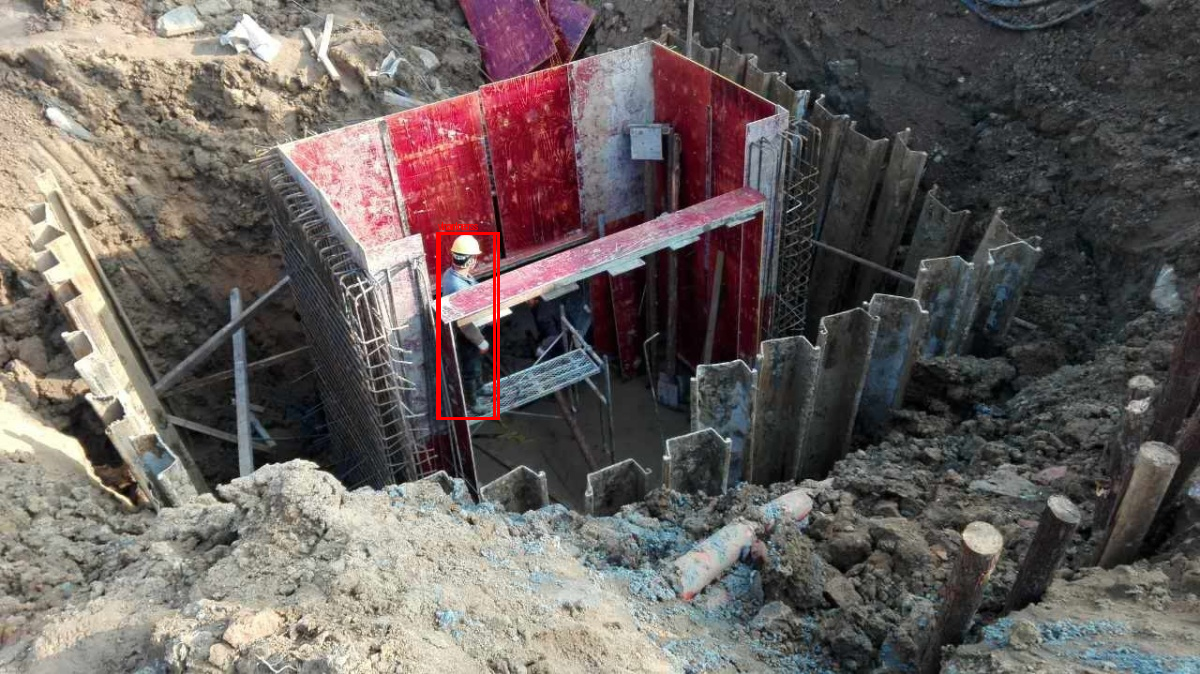
\includegraphics[width=\linewidth]{completeness_before.png}
\caption{Before: the ``worker'' box and ``harness'' box are nearly pixel-identical.}
\end{subfigure}\hfill
\begin{subfigure}{0.44\linewidth}\centering
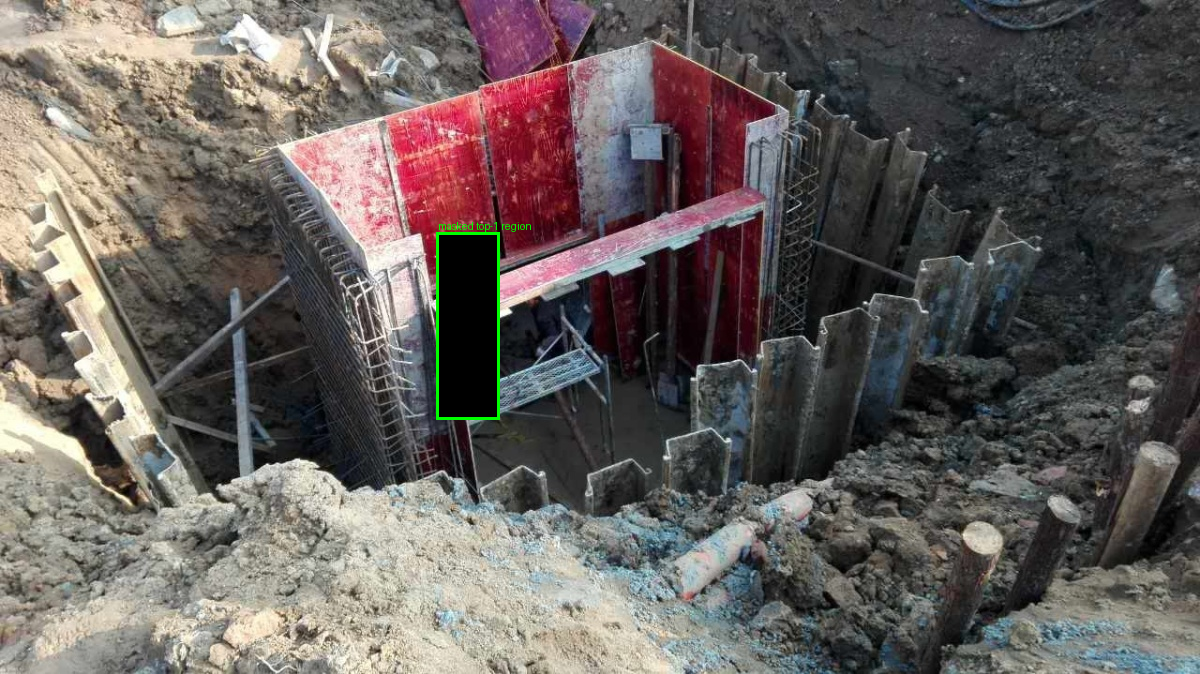
\includegraphics[width=\linewidth]{completeness_after.png}
\caption{After masking the top region: both are erased at once; the answer flips via a fallback, not via
genuine necessity.}
\end{subfigure}
\caption{The worker-fallback artifact that inflates completeness, traced to a specific case.}
\label{fig:completeness}
\end{figure}

\subsection{Efficiency --- is the pipeline affordable at scale?}
The full six-metric pipeline costs \textbf{$\sim$0.5 GPU-hours at $n{=}1{,}000$} on a single RTX 3070
(Figure~\ref{fig:efficiency}). Compute is conclusively \emph{not} the scaling obstacle; every other
issue in this report is about validity, not cost. (The one caveat: this budget is for the current
pipeline; adding gradient-based attribution or dense detection in the full study would change it.)

\begin{figure}[h]
\centering
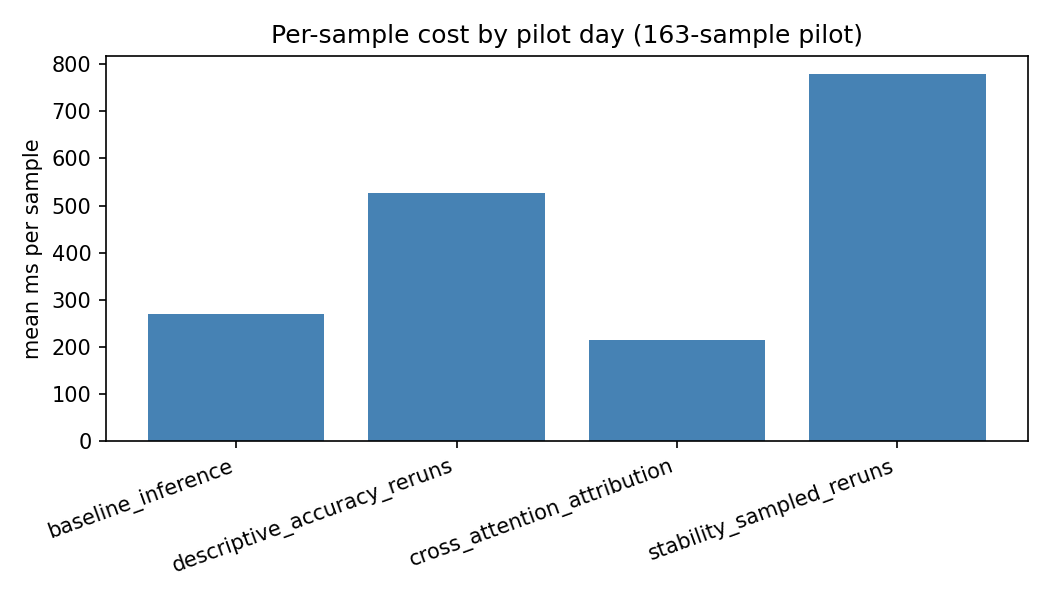
\includegraphics[width=0.62\linewidth]{efficiency.png}
\caption{Per-sample inference cost by pipeline stage. Even summed and extrapolated, the full pipeline is
well under an hour of GPU time per 1,000 samples.}
\label{fig:efficiency}
\end{figure}

\section{Cross-Cutting Findings}
\label{sec:findings}

Reading the metrics together reveals that several ``separate'' weaknesses are one story:

\begin{enumerate}[leftmargin=*,itemsep=3pt]
\item \textbf{One region-ranking choice weakens three metrics at once.} Candidate regions are ranked by
box area as a stand-in for importance (no true saliency signal exists). Because a worker's body box is
almost always larger than the PPE item, the worker is ranked first in 96\% of PPE samples --- so
descriptive accuracy, stability, and completeness all end up testing the worker, not the hard hat,
precisely on the rules the project cares about most. This is the single highest-leverage fix.
\item \textbf{A fallback branch recurs across three tests.} Masking or perturbing the worker can make it
undetectable, rerouting the proxy into a degenerate scene-level branch that flips the answer for reasons
unrelated to the safety concept. The same mechanism appears under deliberate masking, under
perturbation, and inside the completeness check --- found and quantified each time, not left as noise
(Figures~\ref{fig:completeness}, \ref{fig:occlude}).
\item \textbf{Object size confounds two metrics.} Both sparsity and stability partly measure object
footprint rather than explanation quality, because attention-concentration and IoU are both
size-sensitive. This must be controlled before comparing PPE rules to large-object rules.
\item \textbf{The model does not make the judgment.} Florence-2 only returns boxes; a geometric rule
produces the answer. So some metrics measure the proxy, not the model --- the deepest reason to add a
native-VQA model in the full study.
\end{enumerate}

\begin{figure}[h]
\centering
\begin{subfigure}{0.44\linewidth}\centering
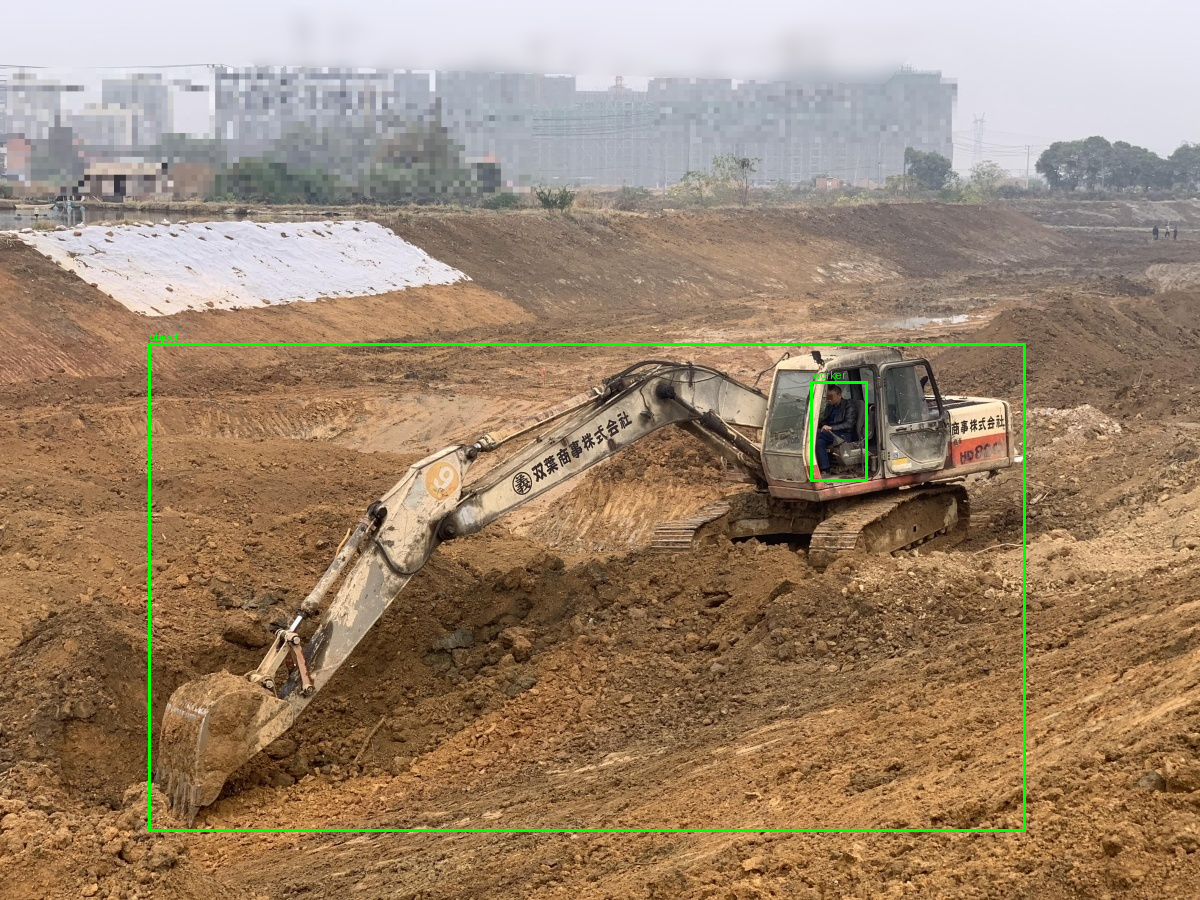
\includegraphics[width=\linewidth]{occlude_fallback_before.png}
\caption{Before: both baseline detections are already wrong but geometrically satisfy the check.}
\end{subfigure}\hfill
\begin{subfigure}{0.44\linewidth}\centering
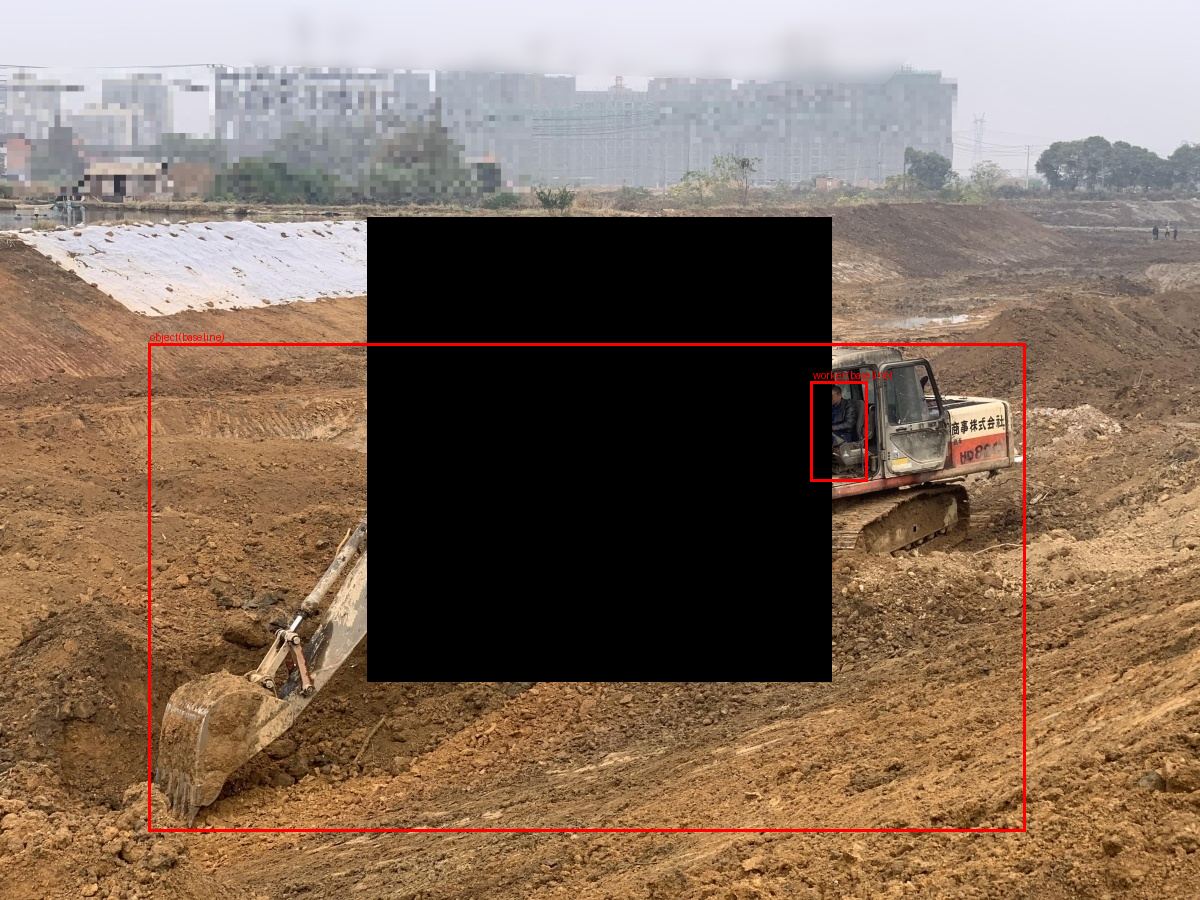
\includegraphics[width=\linewidth]{occlude_fallback_after.png}
\caption{After occlusion: both detections vanish; the answer flips via the fallback, not via genuine
sensitivity to a covered region.}
\end{subfigure}
\caption{The fallback-rerouting mechanism triggered by perturbation rather than by deliberate masking.}
\label{fig:occlude}
\end{figure}

\subsection{Where all six metrics land, side by side}
Figure~\ref{fig:summary} is the cross-metric summary: five per-sample metrics broken down by hazard
class on their own native scales. It is the single figure that most compactly carries the pilot's
quantitative content, and the source the cross-cutting findings were read from.

\begin{figure}[h]
\centering
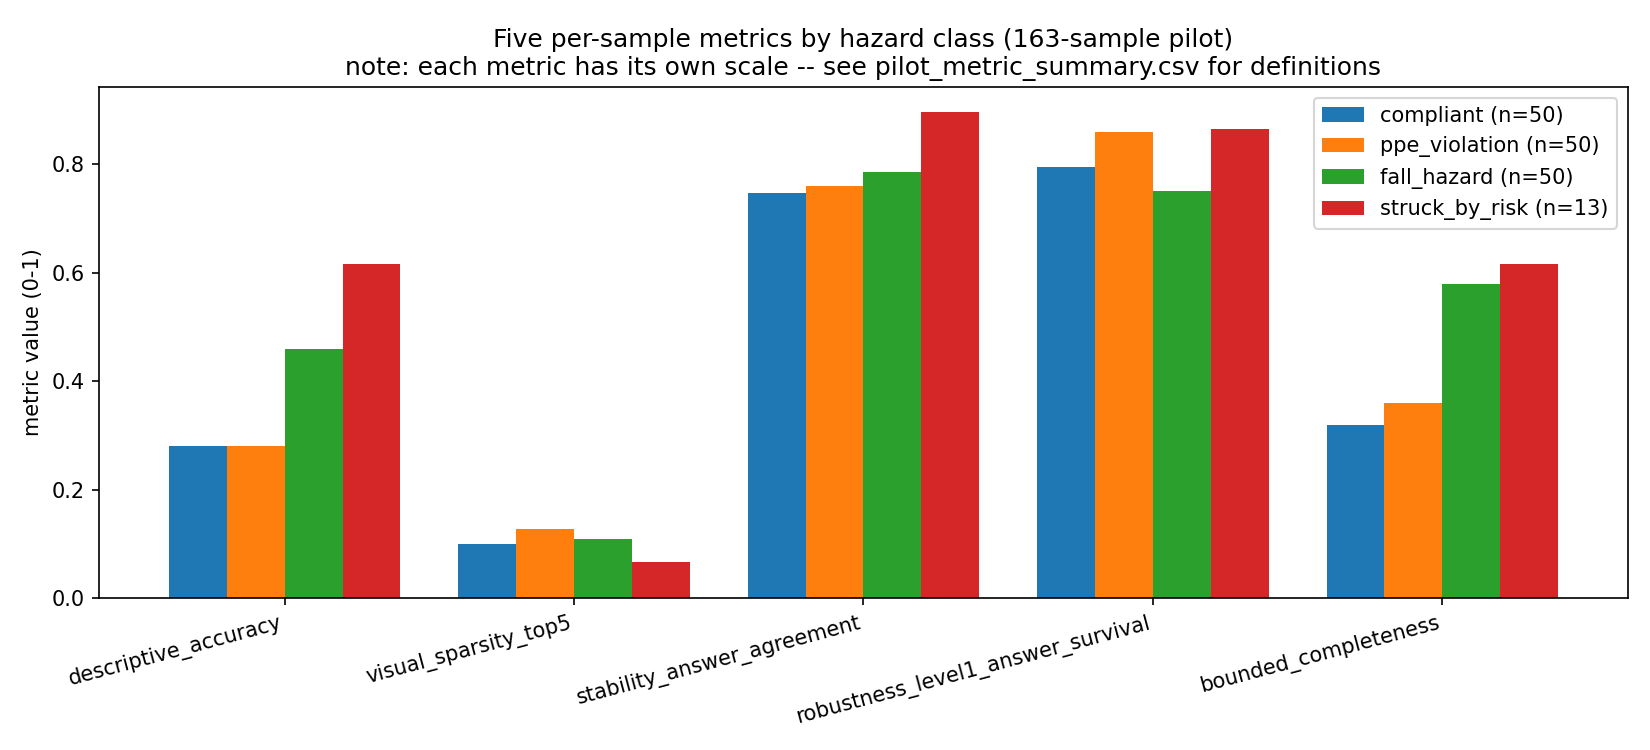
\includegraphics[width=0.95\linewidth]{summary.png}
\caption{Cross-metric summary by hazard class. \code{struck\_by\_risk} rests on $n{=}13$ and should be
read as directional only (see Section~\ref{sec:limits}).}
\label{fig:summary}
\end{figure}

\section{Reproducibility}

The full pipeline was re-run from a clean checkout in a brand-new virtual environment on a fresh
20-sample subset, with zero manual intervention --- every step exited cleanly. The check did more than
confirm reproducibility: because it ran at a different sample size than development, it exposed a real
bug (chart labels hardcoded to the pilot's sample counts) that every prior run had masked. It also hit a
transient dataset-streaming error, auto-recovered, which validated moving the full study to a locally
cached copy of the dataset (now implemented) rather than streaming.

\section{Honest Limitations}
\label{sec:limits}

\begin{itemize}[leftmargin=*,itemsep=2pt]
\item \textbf{Scale:} 163 of 3,004 test images; single model; single GPU.
\item \textbf{\code{struck\_by\_risk} scarcity is a labeling artifact, not a dataset property.} The
mutually-exclusive priority scheme discarded real struck-by images that also had a higher-priority
violation; a direct scan shows the true multi-label pool is $\sim$70 across the full dataset, not 13.
Every \code{struck\_by\_risk} number in this report rests on $n{=}13$ and is directional only.
\item \textbf{The proxy, not the model, makes the judgment} (Section~\ref{sec:findings}), so some metrics
partly measure geometric-rule sensitivity.
\item \textbf{Ranking by area} is an acknowledged stand-in for a true importance signal.
\item \textbf{Single-worker detection}, hardcoded 2D proximity thresholds, bounded (not full)
completeness, Level-1 (plus partial Level-2) robustness only, an uncalibrated confidence proxy, and an
$n{=}4$ adversarial stretch test that is a plausibility probe, not a result.
\item \textbf{Decoding was fragmented} across metrics; the full study should unify it.
\end{itemize}

\section{Scale-Up Direction}
\label{sec:scaleup}

The recommended scale-up is \emph{not} simply ``run 3,004 instead of 163.'' Scaling a biased pipeline
only yields a larger biased sample. The plan (detailed separately) is phased:

\begin{enumerate}[leftmargin=*,itemsep=2pt]
\item \textbf{Foundational fixes first} --- rule-aware region ranking; multi-label class labeling (which
recovers \code{struck\_by\_risk}); bake the worker-loss correction into every metric; split the
rule\_2 prompt concepts; unify decoding. Cheap, high-leverage, unblocks everything.
\item \textbf{Metric-validity fixes} --- size-invariant sparsity and stability; text-token ablation for
descriptive accuracy; severity sweeps for robustness; multi-hazard completeness.
\item \textbf{Reproducibility and statistics} --- containerized environment, multi-seed runs,
minimum-$n$ floors and nonparametric significance tests, programmatically-generated report numbers.
\item \textbf{Attribution} --- keep cross-attention, add integrated gradients as a corroborating second
stream.
\item \textbf{Scope} --- add a native-VQA model (Qwen2.5-VL, in same-proxy \emph{and} native-VQA
comparisons, so the metrics measure model faithfulness), scale ConstructionSite to the full split, and
extend to the SODA (out-of-distribution) and CMA (temporal explanation-stability) datasets.
\end{enumerate}

\subsection*{Six decisions requested of Professor Abdallah}
\begin{enumerate}[leftmargin=*,itemsep=1pt]
\item Is decoder$\to$encoder cross-attention an acceptable stand-in for LRP/DeepLIFT, or is a
transformer-native method required?
\item Minimum-$n$ and statistical-testing standards, especially for the scarce \code{struck\_by\_risk}
class.
\item Approval of the rule-aware region-ranking fix.
\item Full-dataset scaling vs.\ fixing class imbalance first.
\item Scope for a properly powered adversarial-robustness study.
\item Treating rule\_2's two phrasings as distinct physical concepts.
\end{enumerate}

\section{Conclusion}

The six-metric framework transfers from tabular models to a construction-safety VLM: all six metrics ran
end-to-end and produced interpretable, traceable signal, after two adaptations that a feasibility pilot
exists to surface. Just as importantly, the pilot identified exactly what must be fixed before the
numbers can be trusted at scale --- and, in doing so, produced a clear, evidence-backed engineering plan
for a full study whose central aim is to make the metrics measure the model's reasoning rather than the
scaffolding around it.

\end{document}
